\section{Метод тестирования}

Разработанный метод фазинг-тестирования реализует комплексный подход, сочетающий синхронные и асинхронные сценарии для максимального покрытия функционала. Основу методики составляют шесть взаимодополняющих алгоритмов.

\textbf{FsFuzzSubTest1} выполняет работу с отдельным файлом: открытие на чтение, чтение метаданных файла, последовательное чтение блоков данных с перемещением позиции, а затем открытие на запись для записи данных в конец файла. Алгоритм выявляет ошибки управления файловыми дескрипторами, обработки позиционирования и операций ввода-вывода. Обобщенная схема работы алгоритма представлена на рисунке \ref{met:pic:fsfuzzsubtesti}.
\begin{figure}[htbp]
	\centering % Центрирование
	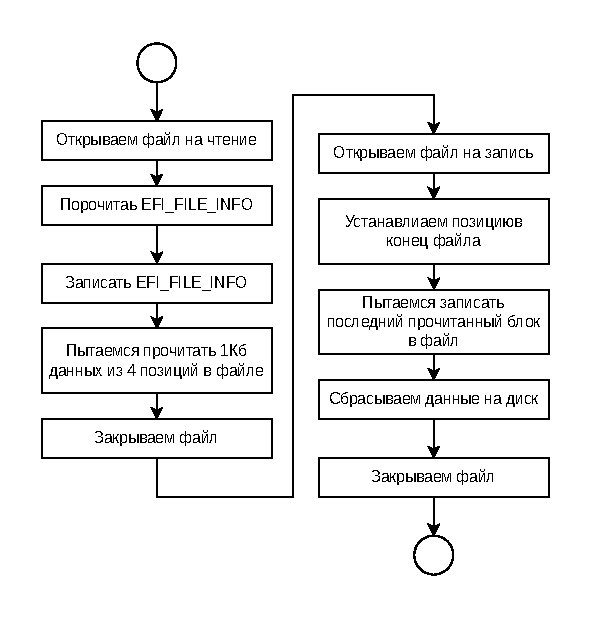
\includegraphics[width=0.5\textwidth]{FsFuzzSubtestI.pdf} % Путь к файлу
	\caption{Обобщенный алгоритм обработки файла \FunName{FsFuzzSubtest1}.} % Подпись
	\label{met:pic:fsfuzzsubtesti} % Метка для ссылок
\end{figure}

\newpage
\textbf{FsFuzzTest1} реализует рекурсивный обход файловой системы с заданной глубиной. Для каждого обнаруженного файла он запускает \FunName{FsFuzzSubtest1}, а для катологов - рекурсивно углубляется в иерархию. Обобщенная схема алгоритма представлена на рисунке \ref{met:pic:fsfuzztesti}.
\begin{figure}[htbp]
	\centering % Центрирование
	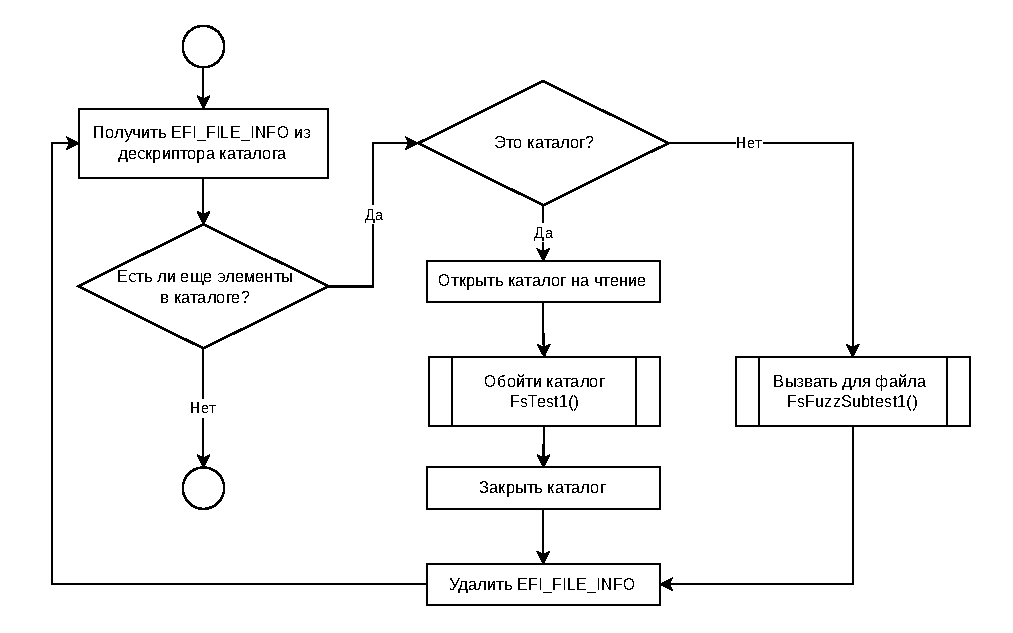
\includegraphics[width=0.7\textwidth]{FsFuzzTestI.pdf} % Путь к файлу
	\caption{Обобщенный алгоритм обхода каталога\FunName{FsFuzzTest1}.} % Подпись
	\label{met:pic:fsfuzztesti} % Метка для ссылок
\end{figure}

\textbf{FsFuzzTest2} последовательно открывает и удаляет все обычные файлы в текущем каталоге. Обобщенная схема алгоритма представлена на рисунке \ref{met:pic:fsfuzztestii}. 
\begin{figure}[htbp]
	\centering % Центрирование
	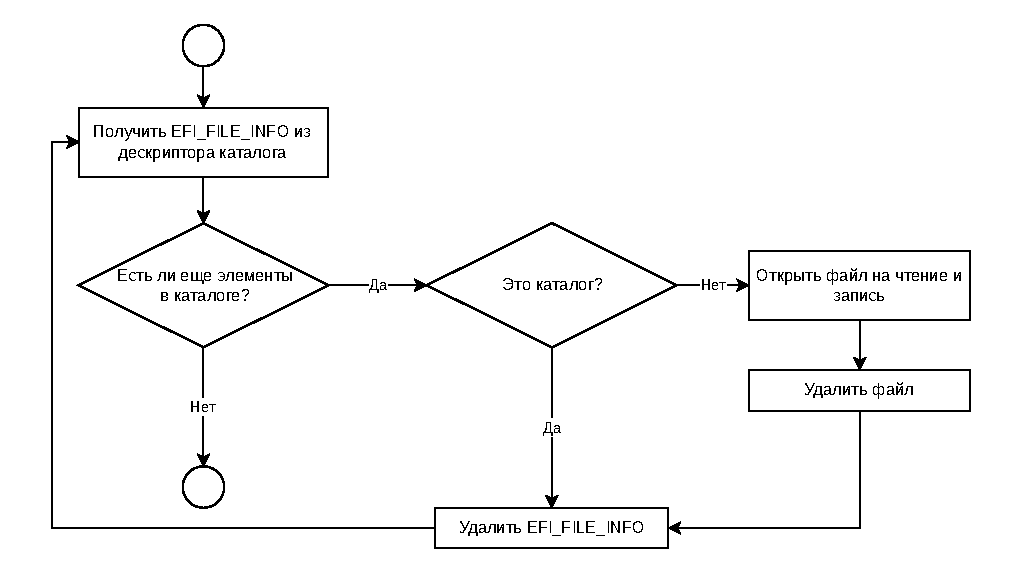
\includegraphics[width=0.7\textwidth]{FsFuzzTestII.pdf} % Путь к файлу
	\caption{Обобщенный алгоритм очистки каталога\FunName{FsFuzzTest2}.} % Подпись
	\label{met:pic:fsfuzztestii} % Метка для ссылок
\end{figure}

\textbf{FsFuzzTest3} создает цепочку вложенных директорий и файл на последнем уровне вложенности. Важно, что алгоритм создает файл, используя длинный путь к нему, но для успешного завершения этой операции необходимо создать все подпапки последовательно. Обобщенная схема алгоритма представлена на рисунке \ref{met:pic:fsfuzztestiii}.
\begin{figure}[h]
	\centering % Центрирование
	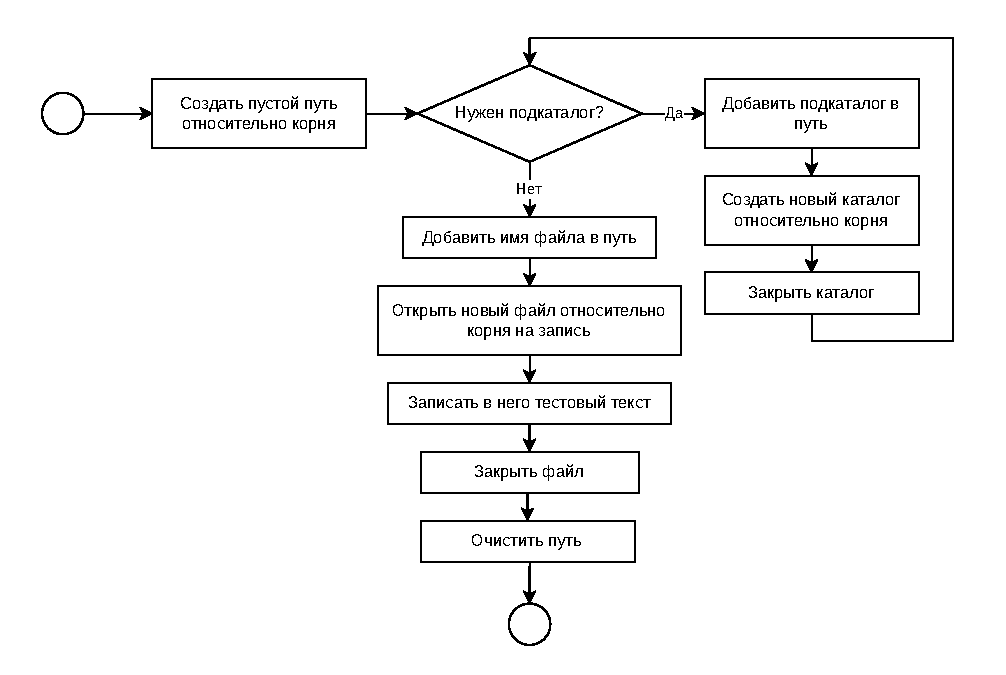
\includegraphics[width=0.7\textwidth]{FsFuzzTestIII.pdf} % Путь к файлу
	\caption{Обобщенный алгоритм создания тестового файла на длинном пути \FunName{FsFuzzTest3}.} % Подпись
	\label{met:pic:fsfuzztestiii} % Метка для ссылок
\end{figure}

\textbf{FsFuzzAsyncWorker} - обработчик результата выполнения асинхронной задачи. После успешного открытия файла в асинхронном режиме он планирует асинхронное чтение из этого файла. После успешного  чтения он планирует асинхронную запись. После успешной записи \FunName{FsFuzzAsyncWorker} помечает асинхронную операцию выполненной, чтобы в дальнейшем освободить все занятые  задачей реурсы. Обобщенная схема алгоритма представлена на рисунке \ref{met:pic:fsfuzzasyncworker}.
\begin{figure}[h]
	\centering % Центрирование
	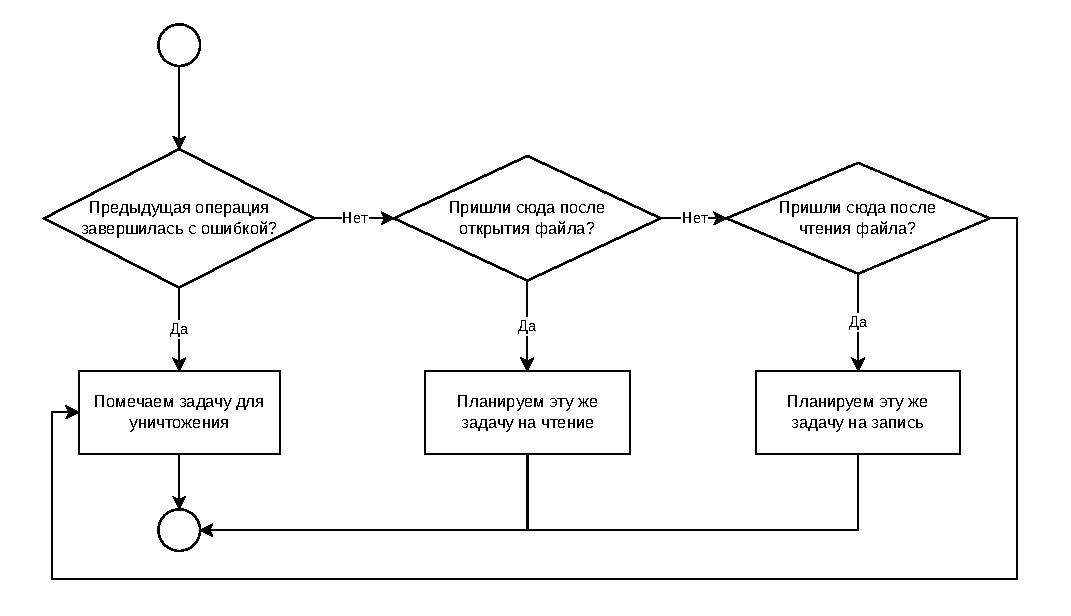
\includegraphics[width=0.7\textwidth]{FsFyzzAsyncWorker.pdf} % Путь к файлу
	\caption{Обобщенный алгоритм обработки асинхронной задачи \FunName{FsFuzzAsyncWorker}.} % Подпись
	\label{met:pic:fsfuzzasyncworker} % Метка для ссылок
\end{figure}

\newpage
\textbf{FsFuzzTest4} дополняет асинхронную проверку, планируя параллельное выполнение операций \FunName{FsFuzzAsyncWorker} для всех файлов в каталоге. Обобщенная схема алгоритма представлена на рисунке \ref{met:pic:fsfuzztestiv}.
\begin{figure}[htbp]
	\centering % Центрирование
	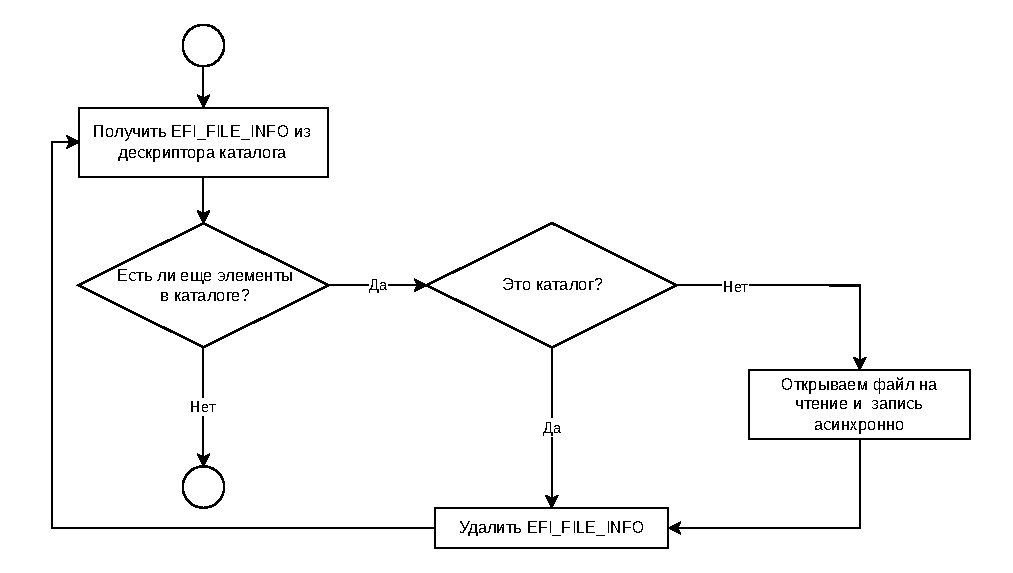
\includegraphics[width=0.7\textwidth]{FsFuzzIV.pdf} % Путь к файлу
	\caption{Обобщенный алгоритм планирования асинхронных операций над файлами из каталога \FunName{FsFuzzTest4}.} % Подпись
	\label{met:pic:fsfuzztestiv} % Метка для ссылок
\end{figure}

Описанные сценарии тестирования используют стандартизированные функции из \VarName{EFI\_FILE\_PROTOCOL} и не вызывают каких-то узкоспециализированные функции драйвера напрямую. Это позволяет применять их для любых драйверов файловых систем без дополнительных правок. Все сценарии последовательно вызываются из главной функции фаззинг-тестирования \FunName{FsFuzzTest}, которая принимает на вход только дескриптор корневого каталога. Алгоритм функции представлен на рисунке \ref{met:pic:fsfuzztest}.
\begin{figure}[htbp]
	\centering % Центрирование
	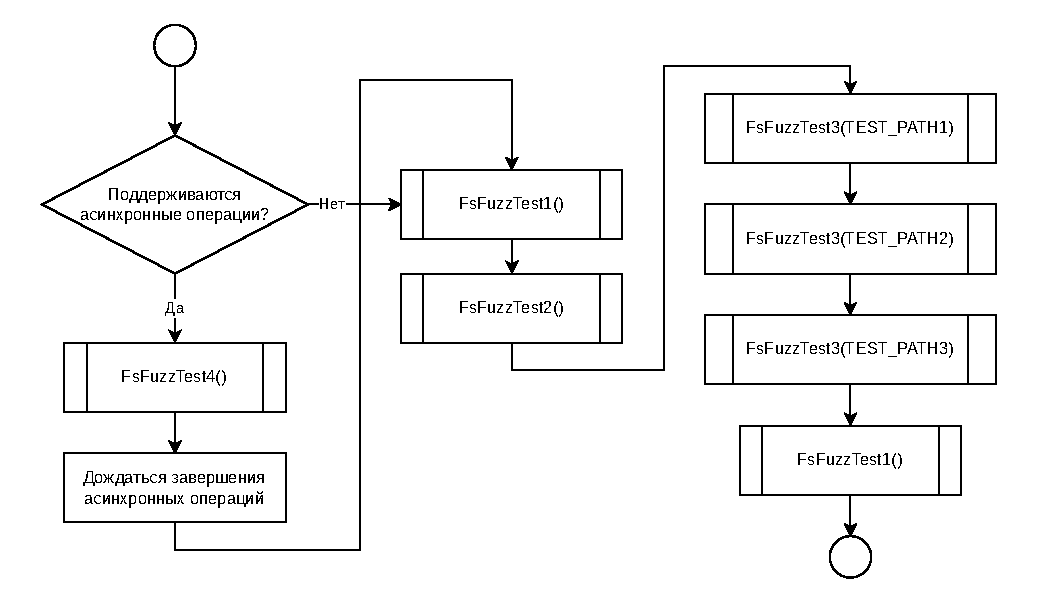
\includegraphics[width=0.75\textwidth]{FsFuzzTest.pdf} % Путь к файлу
	\caption{Главная функция, прводящая фаззинг-тестирование \FunName{FsFuzzTest}.} % Подпись
	\label{met:pic:fsfuzztest} % Метка для ссылок
\end{figure} 

Все перечисленные функции поставляются модулем \textbf{FsFuzzTest}. В завершении на рисунке \ref{met:pic:testscheme} приведена обобщенная схема тестирования драйверов файловой системы, предложенная в этой работе.
\begin{figure}[htbp]
	\centering % Центрирование
	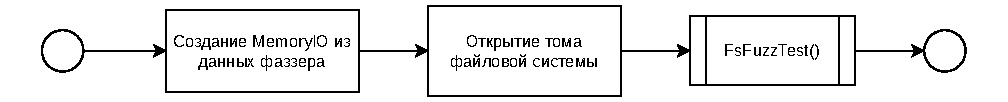
\includegraphics[width=0.8\textwidth]{TestScheme.pdf} % Путь к файлу
	\caption{Полная обобщенная схема предлагаемого метода фаззинг-тестирования.} % Подпись
	\label{met:pic:testscheme} % Метка для ссылок
\end{figure} 